% ============================================================
%  SOAL + PEMBAHASAN  --  FISIKA  --  SSU-ITB 2026
%  SM ITB 2023  (30 soal Fisika) | Paket 8
% ============================================================

\documentclass[11pt]{article}
\usepackage[utf8]{inputenc}
\usepackage[T1]{fontenc}
\usepackage[a4paper,margin=2.5cm,top=2.8cm]{geometry}
\usepackage{amsmath,amssymb}
\usepackage{graphicx}
\usepackage{enumitem}
\usepackage{multicol}
\usepackage{xcolor}
\usepackage[most]{tcolorbox}
\usepackage{fancyhdr}
\usepackage{booktabs}
\usepackage{icomma}
\usepackage{array}

% --- Warna Fisika ---
\definecolor{mapelcolor}{RGB}{20,70,150}
\definecolor{mapelbg}{RGB}{230,238,255}
\definecolor{pembcolor}{RGB}{100,50,130}
\definecolor{pembbg}{RGB}{245,238,252}
\definecolor{gold}{RGB}{210,160,30}

\pagestyle{fancy}\fancyhf{}
\lhead{\small SM ITB 2023 --- Paket 8 --- Pembahasan}
\rhead{\small Fisika}
\cfoot{\small\thepage}
\renewcommand{\headrulewidth}{0.4pt}

\newtcolorbox{soal}[1]{
  breakable,
  colback=mapelbg, colframe=mapelcolor,
  coltitle=white, colbacktitle=mapelcolor,
  fonttitle=\bfseries\sffamily,
  title=Nomor #1,
  boxrule=0.8pt, arc=3pt,
  left=3mm, right=3mm, top=2mm, bottom=2mm}

\newtcolorbox{pembox}{
  breakable,
  colback=pembbg, colframe=pembcolor,
  coltitle=white, colbacktitle=pembcolor,
  fonttitle=\bfseries\sffamily,
  title=Pembahasan,
  boxrule=0.8pt, arc=3pt,
  left=3mm, right=3mm, top=2mm, bottom=2mm}

\newtcolorbox{catatbox}{
  breakable,
  colback=gold!10, colframe=gold!80!black,
  coltitle=white, colbacktitle=gold!80!black,
  fonttitle=\bfseries\sffamily,
  title=Catatan,
  boxrule=0.8pt, arc=3pt,
  left=3mm, right=3mm, top=1.5mm, bottom=1.5mm}

\newcommand{\jawaban}[1]{%
  \noindent\colorbox{gold!30}{\parbox{\dimexpr\linewidth-2\fboxsep\relax}{%
    \textbf{Jawaban:} #1}}\par\smallskip}

\newcommand{\konsep}[1]{\textit{Konsep: #1.}\par\smallskip}

\newenvironment{pil}{%
  \begin{enumerate}[label=(\alph*),leftmargin=*,itemsep=1pt,topsep=3pt]}%
  {\end{enumerate}}
\newenvironment{pilB}{%
  \par\smallskip\begin{multicols}{2}
  \begin{enumerate}[label=(\alph*),leftmargin=*,itemsep=1pt,topsep=3pt]}%
  {\end{enumerate}\end{multicols}}

\newcommand{\gambar}[2][0.50\textwidth]{%
  \begin{center}\includegraphics[width=#1]{#2}\end{center}}

\linespread{1.05}

\begin{document}
\thispagestyle{empty}
\begin{center}
  {\LARGE\bfseries PEMBAHASAN FISIKA}\\[0.4em]
  {\large SM ITB 2023 --- Paket 8}
\end{center}

\vspace{0.4cm}\noindent\textbf{Kunci Jawaban}

\vspace{0.3em}{\small
\begin{tabular}{@{}*{10}{c@{\hspace{1.1em}}}@{}}
\textbf{1}(e)&\textbf{2}(e)&\textbf{3}(a)&\textbf{4}(c)&\textbf{5}(b)&
\textbf{6}(d)&\textbf{7}(d)&\textbf{8}(a)&\textbf{9}(b)&\textbf{10}(b)\\
\end{tabular}

\vspace{0.2em}
\begin{tabular}{@{}*{10}{c@{\hspace{1.1em}}}@{}}
\textbf{11}(c)&\textbf{12}(c)&\textbf{13}(e)&\textbf{14}(c)&\textbf{15}(c)&
\textbf{16}(b)&\textbf{17}(b)&\textbf{18}(c)&\textbf{19}(d)&\textbf{20}(c)\\
\end{tabular}

\vspace{0.2em}
\begin{tabular}{@{}*{10}{c@{\hspace{1.1em}}}@{}}
\textbf{21}(c)&\textbf{22}(b)&\textbf{23}(c)&\textbf{24}(b)&\textbf{25}(b)&
\textbf{26}(b)&\textbf{27}(d)&\textbf{28}(a)&\textbf{29}(c)&\textbf{30}(b)\\
\end{tabular}
}

\clearpage

% ===================================================================
%  SOAL 1 -- 10
% ===================================================================

\begin{soal}{1 -- Gerak Parabola}
Pada saat $t=0$~s, sebuah meriam menembakkan peluru ke udara sehingga peluru bergerak
mengikuti lintasan gerak parabola. Pada saat $2{,}5$~s, posisi peluru tersebut berada pada
$10$~m arah horizontal dan $40$~m arah vertikal dihitung dari posisi awal peluru
ditembakkan. Jika $g=10$~m/s$^2$, peluru jatuh di tanah pada jarak \ldots~m dari posisi meriam.
\begin{pilB}
  \item $42{,}80$ \item $35{,}60$ \item $16{,}40$ \item $62{,}80$ \item $22{,}80$
\end{pilB}
\end{soal}
\begin{pembox}
\konsep{Gerak parabola: komponen horizontal dan vertikal terpisah}
\textbf{Horizontal ($x=v_{0x}t$):}
\[
10 = v_{0x}(2{,}5) \Rightarrow v_{0x} = 4\text{ m/s}.
\]
\textbf{Vertikal ($y=v_{0y}t-\tfrac12gt^2$):}
\[
40 = v_{0y}(2{,}5) - \tfrac12(10)(2{,}5)^2 = 2{,}5\,v_{0y} - 31{,}25
\Rightarrow v_{0y} = 28{,}5\text{ m/s}.
\]
\textbf{Waktu sampai tanah ($y=0$):}
\[
0 = v_{0y}t - 5t^2 = t(v_{0y}-5t)
\Rightarrow t = \frac{28{,}5}{5} = 5{,}7\text{ s}.
\]
\textbf{Jarak horizontal total:}
\[
R = v_{0x}\cdot t = 4(5{,}7) = 22{,}8\text{ m}.
\]
\jawaban{(e) $22{,}80$~m}
\end{pembox}

\begin{soal}{2 -- Kecepatan Sesaat}
Suatu benda bergerak sepanjang sumbu $x$ menurut persamaan $x(t)=4t^2-2t+3$~m.
Kecepatan sesaat pada $t=4$~s adalah \ldots~m/s.
\begin{pilB}
  \item $-16$ \item $24$ \item $65$ \item $0$ \item $30$
\end{pilB}
\end{soal}
\begin{pembox}
\konsep{Kecepatan sesaat = turunan pertama fungsi posisi}
\[
v(t) = \frac{dx}{dt} = 8t - 2.
\]
Pada $t=4$ s:
\[
v(4) = 8(4) - 2 = 32 - 2 = 30\text{ m/s}.
\]
\jawaban{(e) $30$~m/s}
\end{pembox}

\begin{soal}{3 -- Gerak Dua Dimensi}
Benda A dan B bergerak dalam bidang $x$-$y$. $x_A(t)=(t+2)(t-5)$~m; $y_A$ linier dari
$y=-5$~m ($t=0$) ke $y=60$~m ($t=1$~s). $v_{Bx}=v$~m/s, $v_{By}=-5+20t$~m/s. Awalnya
benda berada di tempat yang sama. Nilai $v$ agar benda bertemu kembali adalah \ldots~m/s.
\begin{pilB}
  \item $4$ \item $8$ \item $7$ \item $5$ \item $6$
\end{pilB}
\end{soal}
\begin{pembox}
\konsep{Kesamaan posisi dua benda saat bertemu}
\textbf{Posisi awal:} $x_A(0)=(2)(-5)=-10$~m, $y_A(0)=-5$~m. Benda B mulai di titik yang sama.

\textbf{Fungsi posisi A:} $y_A(t)=-5+65t$ (linier).

\textbf{Fungsi posisi B:} $y_B(t)=-5+\displaystyle\int_0^t(-5+20\tau)\,d\tau=-5-5t+10t^2$.

\textbf{Saat bertemu ($y_A=y_B$):}
\[
-5+65t = -5-5t+10t^2 \Rightarrow 70t = 10t^2 \Rightarrow t=7\text{ s (non-trivial)}.
\]

\textbf{Komponen $x$ saat $t=7$ s:} $x_A(7)=(9)(2)=18$~m.

$x_B(7)=-10+v(7)=18 \Rightarrow 7v=28 \Rightarrow v=4$~m/s.
\jawaban{(a) $4$~m/s}
\end{pembox}

\begin{soal}{4 -- Percepatan pada Lintasan Kurva}
Suatu partikel bergerak pada bidang $x$-$y$ dengan lintasan $y(x)=(2x+6)(x-3)$~m.
Apabila $v_x=0{,}75$~m/s (tetap), maka komponen $y$ dari percepatan partikel sama
dengan \ldots~m/s$^2$.
\begin{pilB}
  \item $3{,}00$ \item $1{,}125$ \item $2{,}25$ \item $1{,}50$ \item $0{,}56$
\end{pilB}
\end{soal}
\begin{pembox}
\konsep{Kinematika: diferensiasi berantai komponen lintasan kurva}
Uraikan lintasan: $y=(2x+6)(x-3)=2x^2-18$, sehingga $\dfrac{dy}{dx}=4x$.

Kecepatan vertikal:
\[
v_y = \frac{dy}{dt} = \frac{dy}{dx}\cdot\frac{dx}{dt} = 4x\cdot v_x = 4x(0{,}75) = 3x.
\]
Percepatan vertikal ($v_x$ tetap $\Rightarrow$ $\dfrac{d^2x}{dt^2}=0$):
\[
a_y = \frac{dv_y}{dt} = 4\frac{dx}{dt}\cdot v_x = 4v_x^2 = 4(0{,}75)^2 = 2{,}25\text{ m/s}^2.
\]
\jawaban{(c) $2{,}25$~m/s$^2$}
\end{pembox}

\begin{soal}{5 -- Kecepatan Rata-Rata}
Posisi partikel $x(t)=t(b-ct)$ dengan $b=20$~m/s dan $c=1$~m/s$^2$. Kecepatan rata-rata
dari $t_1=0$ hingga $t_2=4$~s adalah \ldots~m/s.
\begin{pilB}
  \item $28$ \item $16$ \item $20$ \item $12$ \item $24$
\end{pilB}
\end{soal}
\begin{pembox}
\konsep{Kecepatan rata-rata $=\Delta x/\Delta t$}
$x(t) = bt - ct^2 = 20t - t^2$.

$x(0)=0$; $x(4) = 20(4) - (4)^2 = 80 - 16 = 64$~m.
\[
\bar{v} = \frac{x(4)-x(0)}{4-0} = \frac{64}{4} = 16\text{ m/s}.
\]
\jawaban{(b) $16$~m/s}
\end{pembox}

\begin{soal}{6 -- Percepatan dari Fungsi Posisi}
$x_A(t)=(t+2)(t-5)(t+7)$~m; kecepatan benda B: $v_B(t)=-5+44t$~m/s. Posisi benda A
ketika percepatannya sama dengan percepatan benda B adalah $x=\ldots$~m.
\begin{pilB}
  \item $94$ \item $114$ \item $84$ \item $104$ \item $124$
\end{pilB}
\end{soal}
\begin{pembox}
\konsep{Percepatan = turunan kedua posisi; mencari waktu saat percepatan sama}
Percepatan benda B: $a_B = \dfrac{dv_B}{dt} = 44$~m/s$^2$ (konstan).

Uraikan $x_A$: $(t+2)(t-5)=t^2-3t-10$, sehingga
\[
x_A(t) = (t^2-3t-10)(t+7) = t^3+4t^2-31t-70.
\]
$v_A(t)=3t^2+8t-31$;\quad $a_A(t)=6t+8$.

Saat $a_A=a_B$: $6t+8=44 \Rightarrow t=6$~s.

Posisi A: $x_A(6) = (6+2)(6-5)(6+7) = 8\cdot1\cdot13 = 104$~m.
\jawaban{(d) $104$~m}
\end{pembox}

\begin{soal}{7 -- Dinamika pada Bidang Miring}
Dua balok ($m_1=4$~kg, $m_2=5$~kg) pada bidang miring licin ($45^\circ$ dan $30^\circ$),
dihubungkan tali melalui katrol. Balok $m_2$ ditarik $F=20$~N sejajar bidang ke bawah.
Percepatan balok $m_1$ adalah \ldots~m/s$^2$.
\gambar[0.45\textwidth]{images/8/8-2.png}
\end{soal}
\begin{pembox}
\konsep{Newton II pada sistem dua balok di bidang miring licin}
Ambil arah positif: $m_2$ bergerak turun bidang $30^\circ$, sehingga $m_1$ naik bidang $45^\circ$.

Gaya penggerak total (ke arah positif):
\[
F + m_2 g\sin30^\circ = 20 + 5(10)(0{,}5) = 20 + 25 = 45\text{ N}.
\]
Gaya penahan (komponen berat $m_1$ ke bawah bidang $45^\circ$):
\[
m_1 g\sin45^\circ = 4(10)\!\left(\frac{\sqrt{2}}{2}\right) = 20\sqrt{2} \approx 28{,}28\text{ N}.
\]
Resultan dan massa total sistem:
\[
F_{\text{net}} = 45 - 28{,}28 = 16{,}72\text{ N};\quad m_{\text{tot}} = 4+5 = 9\text{ kg}.
\]
\[
a = \frac{16{,}72}{9} \approx 1{,}86\text{ m/s}^2.
\]
\jawaban{(d) $1{,}86$~m/s$^2$}
\end{pembox}

\begin{soal}{8 -- Gaya Gesek Statis Maksimum}
Balok $40$~kg di meja kasar ($\mu_s=0{,}35$, $\mu_k=0{,}25$) dihubungkan drum kosong
$2$~kg lewat katrol. Air ($\rho=1000$~kg/m$^3$) dimasukkan drum. Volume maksimum air agar
sistem tidak bergerak adalah \ldots
\gambar[0.45\textwidth]{images/8/8-3.png}
\end{soal}
\begin{pembox}
\konsep{Kondisi setimbang: gaya gesek statis maksimum $\geq$ berat drum+air}
Gaya normal pada balok: $N = m_b g = 40(10) = 400$~N.

Gaya gesek statis maksimum: $f_{s,\max} = \mu_s N = 0{,}35(400) = 140$~N.

Berat drum beserta air tidak boleh melebihi $f_{s,\max}$:
\[
(m_d + m_{\text{air}})g \leq 140
\Rightarrow (2 + m_{\text{air}})(10) = 140
\Rightarrow m_{\text{air}} = 12\text{ kg}.
\]
Volume air:
\[
V = \frac{m_{\text{air}}}{\rho} = \frac{12}{1000} = 0{,}012\text{ m}^3 = 12\text{ liter}.
\]
\jawaban{(a) $12$~liter}
\end{pembox}

\begin{soal}{9 -- Gaya Tarik dan Gesekan}
Balok $m=2$~kg diberi gaya $F=20$~N membentuk sudut $\theta$ ($\tan\theta=3/4$) terhadap
sumbu $x$ positif. $\mu_s=0{,}3$, $\mu_k=0{,}2$. Besar percepatan balok adalah \ldots~m/s$^2$.
\gambar[0.45\textwidth]{images/8/8-4.png}
\end{soal}
\begin{pembox}
\konsep{Komponen gaya; cek apakah bergerak; Newton II}
Dari $\tan\theta=3/4$: segitiga 3-4-5, maka $\cos\theta=\tfrac45$, $\sin\theta=\tfrac35$.

(Gaya menekan ke bawah karena sudut di bawah sumbu $x$ --- gambar menunjukkan gaya menekan meja.)

Komponen gaya:
\[
F_x = 20\cdot\frac{4}{5} = 16\text{ N};\quad F_y = 20\cdot\frac{3}{5} = 12\text{ N (ke bawah)}.
\]
Gaya normal: $N = mg + F_y = 2(10)+12 = 32$~N.

Gesek statis maks: $f_{s,\max}=0{,}3(32)=9{,}6$~N $<F_x=16$~N $\Rightarrow$ balok bergerak.

Gesek kinetis: $f_k = 0{,}2(32) = 6{,}4$~N.
\[
a = \frac{F_x - f_k}{m} = \frac{16 - 6{,}4}{2} = \frac{9{,}6}{2} = 4{,}8\text{ m/s}^2.
\]
\jawaban{(b) $4{,}80$~m/s$^2$}
\end{pembox}

\begin{soal}{10 -- Dua Balok Bertumpuk}
Balok A ($20$~kg) di meja licin mendapat gaya $F$, percepatan $6$~m/s$^2$. Balok B ($20$~kg)
bergeser di atas A dengan percepatan $4$~m/s$^2$ (searah). Koefisien gesek A-B $=0{,}4$.
Nilai $F=\ldots$~N.
\gambar[0.45\textwidth]{images/8/8-5.png}
\end{soal}
\begin{pembox}
\konsep{Balok bertumpuk: analisis Newton II tiap balok}
Karena B bergeser relatif terhadap A, gunakan gesek kinetis:
\[
f_k = \mu m_B g = 0{,}4(20)(10) = 80\text{ N}.
\]
Verifikasi percepatan B: $a_B = f_k/m_B = 80/20 = 4$~m/s$^2$ (sesuai soal) ✓

Persamaan Newton II untuk balok A (gaya $F$ ke kanan, gesek B pada A ke kiri):
\[
F - f_k = m_A a_A \Rightarrow F - 80 = 20(6) = 120 \Rightarrow F = 200\text{ N}.
\]
\jawaban{(b) $200$~N}
\end{pembox}

% ===================================================================
%  SOAL 11 -- 20
% ===================================================================

\begin{soal}{11 -- Teorema Usaha-Energi dalam Vektor}
$\vec{F}=(-5\hat{i}+2\hat{j}+3\hat{k})$~N bekerja pada partikel $2$~kg berkecepatan awal
$3$~m/s. Kelajuan partikel setelah perpindahan $\vec{d}=(2\hat{i}+5\hat{j}+\hat{k})$~m
adalah \ldots~m/s.
\begin{pilB}
  \item $4{,}31$ \item $4{,}58$ \item $3{,}46$ \item $3{,}24$ \item $3{,}12$
\end{pilB}
\end{soal}
\begin{pembox}
\konsep{Teorema usaha-energi: $W=\Delta K$; usaha gaya konstan $W=\vec{F}\cdot\vec{d}$}
\[
W = \vec{F}\cdot\vec{d} = (-5)(2)+(2)(5)+(3)(1) = -10+10+3 = 3\text{ J}.
\]
\[
K_i = \tfrac{1}{2}(2)(3)^2 = 9\text{ J};\quad K_f = K_i + W = 9+3 = 12\text{ J}.
\]
\[
v_f = \sqrt{\frac{2K_f}{m}} = \sqrt{\frac{2(12)}{2}} = \sqrt{12} = 2\sqrt{3} \approx 3{,}46\text{ m/s}.
\]
\jawaban{(c) $3{,}46$~m/s}
\end{pembox}

\begin{soal}{12 -- Usaha oleh Gaya Berubah}
Gaya $F(x)=x(k-x)$~N bekerja sepanjang sumbu $x$. Di $x=0$: $K=19$~J; di $x=3$~m:
$K=10$~J. Nilai konstanta $k$ adalah \ldots~N/m.
\begin{pilB}
  \item $4{,}00$ \item $0{,}50$ \item $0$ \item $3{,}00$ \item $1{,}00$
\end{pilB}
\end{soal}
\begin{pembox}
\konsep{Usaha gaya berubah $W=\int F\,dx$; teorema usaha-energi}
\[
W = K_f - K_i = 10 - 19 = -9\text{ J}.
\]
\[
W = \int_0^3(kx-x^2)\,dx = \left[\frac{kx^2}{2}-\frac{x^3}{3}\right]_0^3 = \frac{9k}{2} - 9.
\]
\[
\frac{9k}{2} - 9 = -9 \Rightarrow \frac{9k}{2} = 0 \Rightarrow k = 0.
\]
\jawaban{(c) $k=0$}
\end{pembox}

\begin{soal}{13 -- Usaha Gaya Nonkonservatif}
Balok $2{,}5$~kg meluncur $1$~m pada lintasan miring $\alpha$ ($\tan\alpha=3/4$).
$\mu_s=0{,}50$, $\mu_k=0{,}20$. Usaha gaya nonkonservatif adalah \ldots~J.
\begin{pilB}
  \item $5{,}00$ \item $4{,}00$ \item $-5{,}00$ \item $-3{,}00$ \item $-4{,}00$
\end{pilB}
\end{soal}
\begin{pembox}
\konsep{Gaya nonkonservatif = gesek kinetis; usahanya negatif}
Dari $\tan\alpha=3/4$: $\sin\alpha=3/5$, $\cos\alpha=4/5$.

Gaya normal: $N = mg\cos\alpha = 2{,}5(10)(4/5) = 20$~N.

Gesek kinetis: $f_k = \mu_k N = 0{,}20(20) = 4$~N.

Usaha gesek (arah berlawanan dengan gerak):
\[
W_{\text{gesek}} = -f_k \cdot s = -4(1) = -4\text{ J}.
\]
\jawaban{(e) $-4$~J}
\end{pembox}

\begin{soal}{14 -- Grafik Percepatan dan Gaya}
Dua gaya $F_1$ (bisa diputar sudut $\theta$) dan $F_2$ (tetap, arah $x$) pada benda
$1{,}5$~kg di lantai licin. Grafik: $a_x(\theta=0^\circ)=A=3$~m/s$^2$;
$a_x(\theta=90^\circ)=A/3$. Besar gaya $F_2$ adalah \ldots~N.
\gambar[0.55\textwidth]{images/8/8-6.png}
\end{soal}
\begin{pembox}
\konsep{Newton II pada sumbu $x$; saat $\theta=90^\circ$ komponen $x$ dari $F_1$ nol}
Pada $\theta=90^\circ$: $F_{1x}=F_1\cos90^\circ=0$, sehingga hanya $F_2$ yang bekerja pada sumbu $x$:
\[
a_x(90^\circ) = \frac{F_2}{m} = \frac{A}{3} = \frac{3}{3} = 1\text{ m/s}^2.
\]
\[
F_2 = m\cdot a_x(90^\circ) = 1{,}5(1) = 1{,}5\text{ N}.
\]
\jawaban{(c) $1{,}50$~N}
\end{pembox}

\begin{soal}{15 -- Tegangan Tali pada Dua Balok}
Benda A ($2$~kg) dan B ($6$~kg) di meja licin, dihubungkan tali. Gaya $F_A=10$~N ($30^\circ$)
pada A; gaya $F_B=40$~N ($30^\circ$) pada B. Tegangan tali adalah \ldots~N.
\gambar[0.55\textwidth]{images/8/8-7.png}
\end{soal}
\begin{pembox}
\konsep{Newton II sistem; pisah analisis tiap benda untuk tegangan tali}
Komponen horizontal kedua gaya (meja licin, tak ada gesekan):
\[
F_{Ax} = 10\cos30^\circ = 5\sqrt{3}\text{ N};\quad F_{Bx} = 40\cos30^\circ = 20\sqrt{3}\text{ N}.
\]
Keduanya searah kanan. Percepatan sistem:
\[
a = \frac{F_{Ax}+F_{Bx}}{m_A+m_B} = \frac{25\sqrt{3}}{8}\text{ m/s}^2.
\]
Untuk balok A (Newton II; $F_{Ax}$ ke kanan, tegangan $T$ ke kanan dari tali ke B):

\textit{Catatan:} Benda B menggerakkan sistem, tali menarik A ke arah B. Tinjau balok A saja:
\[
F_{Ax} + T = m_A a \Rightarrow T = m_A a - F_{Ax}
= 2\cdot\frac{25\sqrt{3}}{8} - 5\sqrt{3}
= \frac{25\sqrt{3}}{4} - 5\sqrt{3} = \frac{5\sqrt{3}}{4} \approx 2{,}17\text{ N}.
\]
\jawaban{(c) $2{,}17$~N}
\end{pembox}

\begin{soal}{16 -- Persamaan Gerak Harmonik Sederhana}
Partikel GHS amplitudo $A$. Pada $t=0$: $x=-A/2$ dan bergerak ke arah $x$ positif.
Persamaan simpangan yang sesuai adalah \ldots
\begin{pil}
  \item $x=A\sin(\omega t+\pi/6)$
  \item $x=A\sin(\omega t-\pi/6)$
  \item $x=A\cos(\omega t+\pi/3)$
  \item $x=-A\cos(\omega t-\pi/3)$
  \item $x=A\cos(\omega t-\pi/6)$
\end{pil}
\end{soal}
\begin{pembox}
\konsep{Uji dua syarat: $x(0)=-A/2$ dan $v(0)>0$}
Uji pilihan (b), $x=A\sin\!\left(\omega t-\dfrac{\pi}{6}\right)$:
\[
x(0) = A\sin\!\left(-\frac{\pi}{6}\right) = -\frac{A}{2}\checkmark
\]
\[
v(t) = A\omega\cos\!\left(\omega t-\frac{\pi}{6}\right);\quad
v(0) = A\omega\cos\!\left(-\frac{\pi}{6}\right) = A\omega\cdot\frac{\sqrt{3}}{2} > 0\checkmark
\]
Kedua syarat terpenuhi.
\jawaban{(b) $x=A\sin\!\left(\omega t-\dfrac{\pi}{6}\right)$}
\end{pembox}

\begin{soal}{17 -- Daya dan Efisiensi}
Pendaki $50$~kg mendaki $\Delta h=1{,}5$~km dalam $4$~jam. Efisiensi tubuh $10\%$.
Daya masukan yang dibutuhkan adalah \ldots
\begin{pilB}
  \item $0{,}58$~W \item $520{,}83$~W \item $57{,}87$~W \item $5{,}21$~W \item $578{,}70$~W
\end{pilB}
\end{soal}
\begin{pembox}
\konsep{Efisiensi: $\eta = P_{\text{berguna}}/P_{\text{masukan}}$}
Energi berguna (melawan gravitasi):
\[
E = mg\Delta h = 50(10)(1500) = 750\,000\text{ J}.
\]
Waktu: $t=4\times3600=14\,400$~s.
\[
P_{\text{berguna}} = \frac{E}{t} = \frac{750\,000}{14\,400} \approx 52{,}08\text{ W}.
\]
\[
P_{\text{masukan}} = \frac{P_{\text{berguna}}}{\eta} = \frac{52{,}08}{0{,}10} \approx 520{,}83\text{ W}.
\]
\jawaban{(b) $520{,}83$~W}
\end{pembox}

\begin{soal}{18 -- Gelombang pada Dawai}
Dawai gitar $L=0{,}8$~m, $m=8$~g menghasilkan harmonik ketiga (nada atas kedua) dengan
frekuensi $300$~Hz. Besar tegangan pada dawai adalah \ldots
\begin{pilB}
  \item $128$~N \item $160$~N \item $256$~N \item $320$~N \item $640$~N
\end{pilB}
\end{soal}
\begin{pembox}
\konsep{Frekuensi harmonik dawai; cepat rambat gelombang dan tegangan}
Harmonik ketiga ($n=3$):
\[
f_3 = \frac{3v}{2L} \Rightarrow v = \frac{2Lf_3}{3} = \frac{2(0{,}8)(300)}{3} = 160\text{ m/s}.
\]
Massa jenis linear: $\mu = m/L = 0{,}008/0{,}8 = 0{,}01$~kg/m.
\[
T = \mu v^2 = 0{,}01(160)^2 = 0{,}01(25600) = 256\text{ N}.
\]
\jawaban{(c) $256$~N}
\end{pembox}

\begin{soal}{19 -- Ayunan dengan Gaya Gesek}
Orang $60$~kg mengayun pada tali $L=3{,}5$~m dari sudut $30^\circ$ (dari vertikal)
dengan keadaan diam. Gaya gesek konstan $60$~N berlawanan kecepatan. Laju di titik
terendah adalah \ldots~m/s.
\begin{center}
  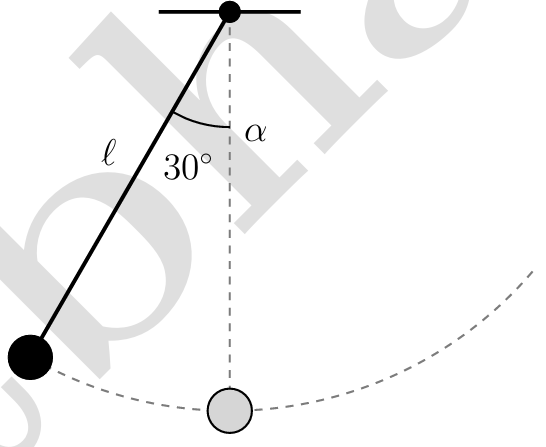
\includegraphics[width=0.28\textwidth]{images/8/8-8.png}\hfill
  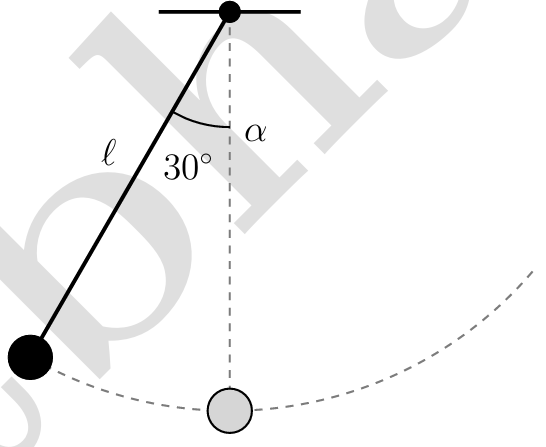
\includegraphics[width=0.28\textwidth]{images/8/8-9.png}
\end{center}
\end{soal}
\begin{pembox}
\konsep{Energi mekanik + usaha gaya non-konservatif (gesek)}
Penurunan ketinggian dari $\theta=30^\circ$ ke titik terendah:
\[
h = L(1-\cos30^\circ) = 3{,}5\!\left(1-\frac{\sqrt{3}}{2}\right) \approx 3{,}5(0{,}1340) = 0{,}4699\text{ m}.
\]
Energi potensial yang dilepas:
\[
\Delta EP = mgh = 60(10)(0{,}4699) = 281{,}9\text{ J}.
\]
Panjang busur lintasan:
\[
s = L\theta = 3{,}5\cdot\frac{\pi}{6} \approx 1{,}833\text{ m}.
\]
Usaha gesek (negatif):
\[
W_f = -f\cdot s = -60(1{,}833) = -110{,}0\text{ J}.
\]
Energi kinetik di titik terendah:
\[
K_f = \Delta EP + W_f = 281{,}9 - 110{,}0 = 171{,}9\text{ J}.
\]
\[
v = \sqrt{\frac{2K_f}{m}} = \sqrt{\frac{2(171{,}9)}{60}} = \sqrt{5{,}73} \approx 2{,}39\text{ m/s}.
\]
\jawaban{(d) $2{,}39$~m/s}
\end{pembox}

\begin{soal}{20 -- Superposisi Getaran Harmonik}
$y_1=6\sin20t$ cm dan $y_2=8\cos20t$ cm. Jika resultan $y=R\sin(20t+\varphi)$,
amplitudo resultan $R$ adalah \ldots
\begin{pilB}
  \item $14$~cm \item $12$~cm \item $10$~cm \item $8$~cm \item $2$~cm
\end{pilB}
\end{soal}
\begin{pembox}
\konsep{Penjumlahan fasor: sin dan cos berbeda fase $90^\circ$}
$y_2=8\cos20t=8\sin(20t+90^\circ)$. Kedua komponen saling tegak lurus:
\[
R = \sqrt{6^2 + 8^2} = \sqrt{36+64} = \sqrt{100} = 10\text{ cm}.
\]
\jawaban{(c) $10$~cm}
\end{pembox}

% ===================================================================
%  SOAL 21 -- 30
% ===================================================================

\begin{soal}{21 -- Efek Doppler pada Bunyi Pantul}
Mobil pemadam bergerak menuju dinding, sirene $680$~Hz. Pengemudi mendengar bunyi pantul
$760$~Hz. Cepat rambat bunyi $340$~m/s. Kelajuan mobil adalah \ldots
\begin{pil}
  \item $54$~km/jam \item $60$~km/jam \item $68$~km/jam \item $72$~km/jam \item $90$~km/jam
\end{pil}
\end{soal}
\begin{pembox}
\konsep{Efek Doppler dua tahap: sumber bergerak ke dinding, dinding pantulkan ke sumber}
Untuk bunyi pantul dari dinding diam yang didengar pengemudi (sumber dan pengamat bergerak menuju reflector):
\[
f' = f\cdot\frac{v+u}{v-u}
\]
dengan $u$ kelajuan mobil, karena mobil menuju dinding (sumber mendekati) dan mendengar pantul (pengamat mendekati).
\[
760 = 680\cdot\frac{340+u}{340-u}
\Rightarrow \frac{760}{680} = \frac{19}{17} = \frac{340+u}{340-u}.
\]
Kalikan silang:
\[
19(340-u) = 17(340+u)
\Rightarrow 6460 - 19u = 5780 + 17u
\Rightarrow 36u = 680
\Rightarrow u = \frac{680}{36} \approx 18{,}89\text{ m/s}.
\]
Konversi: $u = 18{,}89 \times 3{,}6 \approx 68$~km/jam.
\jawaban{(c) $68$~km/jam}
\end{pembox}

\begin{soal}{22 -- Gerak Rotasi Diperlambat}
Motor memutar roda pada $90$ rpm, dimatikan dengan perlambatan $2$~rad/s$^2$.
Waktu yang diperlukan roda untuk berhenti adalah \ldots~s.
\begin{pilB}
  \item $6{,}17$ \item $4{,}71$ \item $2{,}09$ \item $6{,}23$ \item $5{,}24$
\end{pilB}
\end{soal}
\begin{pembox}
\konsep{Kinematika rotasi: $\omega=\omega_0-\alpha t$}
Ubah kecepatan sudut awal: $90$~rpm $= \dfrac{90}{60} = 1{,}5$~rps.
\[
\omega_0 = 1{,}5 \times 2\pi = 3\pi\text{ rad/s} \approx 9{,}42\text{ rad/s}.
\]
Roda berhenti saat $\omega=0$:
\[
0 = \omega_0 - \alpha t
\Rightarrow t = \frac{\omega_0}{\alpha} = \frac{3\pi}{2} \approx 4{,}71\text{ s}.
\]
\jawaban{(b) $4{,}71$~s}
\end{pembox}

\begin{soal}{23 -- Susunan Pegas dan Frekuensi}
Tiga pegas identik ($k$). Sistem P: dua seri lalu diparalel dengan satu. Sistem Q: dua
paralel lalu diseri dengan satu. Massa $m$ sama. Perbandingan $f_P:f_Q$ adalah \ldots
\begin{pilB}
  \item $1:2$ \item $\sqrt{2}:1$ \item $3:2$ \item $2:3$ \item $1:\sqrt{2}$
\end{pilB}
\end{soal}
\begin{pembox}
\konsep{Konstanta pegas ekuivalen; frekuensi $f\propto\sqrt{k_{\text{eq}}}$}
\textbf{Sistem P:} dua seri $\Rightarrow k_s=k/2$; diparalel dengan $k$:
\[
k_P = \frac{k}{2} + k = \frac{3k}{2}.
\]
\textbf{Sistem Q:} dua paralel $\Rightarrow k_p=2k$; diseri dengan $k$:
\[
k_Q = \frac{(2k)(k)}{2k+k} = \frac{2k}{3}.
\]
\[
\frac{f_P}{f_Q} = \sqrt{\frac{k_P}{k_Q}} = \sqrt{\frac{3k/2}{2k/3}} = \sqrt{\frac{9}{4}} = \frac{3}{2}.
\]
\jawaban{(c) $3:2$}
\end{pembox}

\begin{soal}{24 -- Cepat Rambat Bunyi dalam Fluida}
$v=\sqrt{B/\rho}$. Pernyataan:
(1) Semakin besar $B$, bunyi merambat semakin cepat.
(2) $B$ tetap, semakin besar $\rho$, bunyi semakin lambat.
(3) Tegangan permukaan adalah besaran utama penentu $v$ bunyi di fluida homogen.
(4) Fluida sukar dimampatkan cenderung $v$ lebih besar.
Pernyataan yang benar adalah \ldots
\begin{pil}
  \item (1) dan (2) \item (1), (2), dan (4)
  \item (2) dan (3) \item (3) dan (4) \item (1), (2), (3), dan (4)
\end{pil}
\end{soal}
\begin{pembox}
\konsep{Analisis rumus $v=\sqrt{B/\rho}$ dan fisika fluida}

(1) \textbf{Benar} --- $v\propto\sqrt{B}$, jadi semakin besar $B$ semakin cepat.

(2) \textbf{Benar} --- $v\propto 1/\sqrt{\rho}$, jadi semakin besar $\rho$ semakin lambat.

(3) \textbf{Salah} --- Tegangan permukaan bukan penentu utama cepat rambat bunyi di fluida homogen; yang menentukan adalah modulus bulk dan massa jenis.

(4) \textbf{Benar} --- Fluida sukar dimampatkan memiliki modulus bulk $B$ besar, sehingga $v$ lebih besar.

Yang benar: (1), (2), dan (4).
\jawaban{(b) (1), (2), dan (4)}
\end{pembox}

\begin{soal}{25 -- Pusat Massa Empat Benda}
Benda $n$ ($n=1,2,3,4$): $\vec{r}_n(t)=\dfrac{n}{2}\vec{v}+\vec{a}\,t$;
$\vec{v}=(4\hat{i}+2\hat{j})$~m/s, $\vec{a}=-5\hat{j}$~m/s$^2$; awal di pusat koordinat.
Posisi pusat massa pada $t=1$~s adalah \ldots~m.
\begin{pil}
  \item $2\hat{i}-4\hat{j}$ \item $5\hat{i}-2{,}5\hat{j}$
  \item $1{,}5\hat{i}-4{,}25\hat{j}$ \item $2{,}5\hat{i}-3{,}75\hat{j}$ \item $0{,}5\hat{i}-4{,}75\hat{j}$
\end{pil}
\end{soal}
\begin{pembox}
\konsep{Pusat massa: rata-rata posisi (massa sama); substitusi $t=1$ s}
Pada $t=1$ s: $\vec{r}_n(1) = \dfrac{n}{2}\vec{v}+\vec{a}$.

Rata-rata $\dfrac{n}{2}$ untuk $n=1,2,3,4$:
\[
\overline{\!\frac{n}{2}\!} = \frac{\tfrac12+1+\tfrac32+2}{4} = \frac{\tfrac{10}{2}}{4} = \frac{5}{4} = 1{,}25.
\]
\[
\vec{r}_{\text{PM}} = 1{,}25\,\vec{v} + \vec{a}
= 1{,}25(4\hat{i}+2\hat{j}) + (-5\hat{j})
= 5\hat{i} + 2{,}5\hat{j} - 5\hat{j}
= 5\hat{i} - 2{,}5\hat{j}\text{ m}.
\]
\jawaban{(b) $5\hat{i}-2{,}5\hat{j}$~m}
\end{pembox}

\begin{soal}{26 -- Efek Doppler Pengamat Menjauh}
Drone diam, alarm $500$~Hz. Pelari menjauhi drone, kelajuan $10$~m/s. Cepat rambat bunyi
$340$~m/s. Frekuensi yang didengar pelari adalah \ldots
\begin{pilB}
  \item $470{,}6$~Hz \item $485{,}3$~Hz \item $500{,}0$~Hz \item $514{,}7$~Hz \item $529{,}4$~Hz
\end{pilB}
\end{soal}
\begin{pembox}
\konsep{Efek Doppler: sumber diam, pengamat menjauhi}
\[
f' = f\cdot\frac{v - v_o}{v}
= 500\cdot\frac{340 - 10}{340}
= 500\cdot\frac{330}{340}
= 500(0{,}9706) \approx 485{,}3\text{ Hz}.
\]
\jawaban{(b) $485{,}3$~Hz}
\end{pembox}

\begin{soal}{27 -- Periode Osilasi dari Energi Potensial}
Benda $2$~kg berosilasi pada pegas licin; $U=25x^2$ (J; $x$ dalam m). Periode osilasi
adalah \ldots
\begin{pil}
  \item $\dfrac{\pi}{10}$~s \item $\dfrac{\pi}{5}$~s \item $\dfrac{\pi}{\sqrt{2}}$~s
  \item $\dfrac{2\pi}{5}$~s \item $\pi$~s
\end{pil}
\end{soal}
\begin{pembox}
\konsep{$U=\tfrac12kx^2$; ekstrak $k$; gunakan $T=2\pi\sqrt{m/k}$}
\[
U = \frac{1}{2}kx^2 = 25x^2 \Rightarrow k = 50\text{ N/m}.
\]
\[
T = 2\pi\sqrt{\frac{m}{k}} = 2\pi\sqrt{\frac{2}{50}} = 2\pi\sqrt{\frac{1}{25}} = \frac{2\pi}{5}\text{ s}.
\]
\jawaban{(d) $\dfrac{2\pi}{5}$~s}
\end{pembox}

\begin{soal}{28 -- Pernyataan tentang Getaran Pegas}
Pegas bergetar $15$ kali dalam $12$~s. Pernyataan:
(1) $T=0{,}8$~s; (2) $f=1{,}25$~Hz; (3) waktu setimbang ke amplitudo $=0{,}20$~s;
(4) percepatan maks di titik setimbang. Yang benar adalah \ldots
\begin{pil}
  \item (1), (2), dan (3) \item (1) dan (3)
  \item (2) dan (4) \item (4) saja \item (1), (2), (3), dan (4)
\end{pil}
\end{soal}
\begin{pembox}
\konsep{Besaran-besaran GHS dari data jumlah getaran dan waktu}
$f = \dfrac{N}{t} = \dfrac{15}{12} = 1{,}25$~Hz. \quad\textbf{(2) Benar.}

$T = \dfrac{1}{f} = \dfrac{1}{1{,}25} = 0{,}8$~s. \quad\textbf{(1) Benar.}

Waktu dari titik setimbang ke amplitudo maksimum $= \dfrac{T}{4} = \dfrac{0{,}8}{4} = 0{,}20$~s. \quad\textbf{(3) Benar.}

Percepatan GHS: $a=-\omega^2x$. Percepatan maksimum saat $|x|$ maksimum (di simpangan maksimum), \textbf{bukan} di titik setimbang. \quad\textbf{(4) Salah.}

Yang benar: (1), (2), dan (3).
\jawaban{(a) (1), (2), dan (3)}
\end{pembox}

\begin{soal}{29 -- Tegangan Tali dari Persamaan Gelombang}
Gelombang transversal: $y=0{,}04\sin(\pi x-40\pi t)$ ($x,y$ dalam m, $t$ dalam s).
Massa jenis linear tali $\mu=2\times10^{-3}$~kg/m. Tegangan tali adalah \ldots
\begin{pilB}
  \item $1{,}6$~N \item $2{,}4$~N \item $3{,}2$~N \item $4{,}0$~N \item $6{,}4$~N
\end{pilB}
\end{soal}
\begin{pembox}
\konsep{Identifikasi $k$ dan $\omega$ dari persamaan gelombang; $v=\omega/k$; $T=\mu v^2$}
Dari bentuk $y=A\sin(kx-\omega t)$: $k=\pi$~rad/m, $\omega=40\pi$~rad/s.
\[
v = \frac{\omega}{k} = \frac{40\pi}{\pi} = 40\text{ m/s}.
\]
\[
T = \mu v^2 = (2\times10^{-3})(40)^2 = (2\times10^{-3})(1600) = 3{,}2\text{ N}.
\]
\jawaban{(c) $3{,}2$~N}
\end{pembox}

\begin{soal}{30 -- Usaha dan Energi pada Bidang Miring Licin}
Balok $4$~kg ditarik $F=24$~N sejajar bidang miring licin ($30^\circ$). Mulai dari diam.
Kelajuan setelah menempuh $2$~m adalah \ldots~m/s.
\begin{pilB}
  \item $2{,}83$ \item $2{,}00$ \item $4{,}00$ \item $5{,}66$ \item $3{,}74$
\end{pilB}
\end{soal}
\begin{pembox}
\konsep{Newton II pada bidang miring; kinematika $v^2=2as$}
Komponen berat sepanjang bidang (ke bawah): $mg\sin30^\circ = 4(10)(0{,}5) = 20$~N.

Resultan gaya sepanjang bidang:
\[
\Sigma F = F - mg\sin30^\circ = 24 - 20 = 4\text{ N}.
\]
Percepatan: $a = \Sigma F/m = 4/4 = 1$~m/s$^2$.

Dari keadaan diam ($v_0=0$), menempuh $s=2$~m:
\[
v^2 = 2as = 2(1)(2) = 4 \Rightarrow v = 2\text{ m/s}.
\]
\jawaban{(b) $2{,}00$~m/s}
\end{pembox}

\end{document}
